\documentclass[sigconf,nonacm]{acmart}

\usepackage[T1]{fontenc}
\usepackage{graphicx}
\usepackage{url}

\title{What Google Knows: Measuring Telemetry and Identifier Exposure Across Privacy-Focused Android Operating Systems}

\author{Bruno Mirčevski}
\orcid{0009-0007-1008-6708}
\affiliation{%
  \institution{Faculty of Computer Science, Bialystok University of Technology}
  \city{Bialystok}
  \country{Poland}
}

\author{Krzysztof Jurczuk}
\orcid{0000-0001-6469-1769}
\affiliation{%
  \institution{Faculty of Computer Science, Bialystok University of Technology}
  \city{Bialystok}
  \country{Poland}
}

\begin{document}

\begin{abstract}
This paper presents a comparative analysis of user privacy in Android operating systems through network traffic inspection. Using a controlled man-in-the-middle setup and traffic decryption techniques, six Android systems were evaluated: stock Android (GMS), GrapheneOS, iod\'eOS, and three variants of LineageOS (stock, Gapps, microG). While prior work focuses on applications or stock Android across device manufacturers, this study investigates alternative Android distributions designed with privacy as a primary objective. We examined outbound connections, transmitted identifiers, and network traffic patterns to assess the impact of integrated Google services on user privacy.
\end{abstract}

\keywords{Android, Privacy, Network traffic}

\maketitle

\section{Introduction}
Android is the dominant mobile operating system and acts as a primary gateway to the digital world for billions of users. It is crucial for the core operating system to be a reliable, stable, and trustworthy platform that allows users to run applications and services of their choice. While third-party application privacy has been widely studied \cite{appDataCollection1,appDataCollection2,appDataCollection3,appDataCollection4}, less attention is typically paid to the operating system layer and to privileged service frameworks that silently enable additional functionality.

While the Android core is the Android Open Source Project (AOSP), most consumer devices include GMS (Google Mobile Services) layered on top. They are implemented as privileged system applications to provide baseline functionality. Application developers commonly assume their presence by default. This design tightly couples many functions into a single service stack. Enabling useful capabilities may implicitly enable others that a user would not choose, such as advertising identifiers, telemetry, and behavioral tracking. Because Google’s business model is strongly advertising-driven, many users may be unwilling to entrust this provider with broad access to their devices and data.

In principle, users should be able to choose which services they rely on and have confidence that these choices are enforced by the platform’s permission and isolation mechanisms. This demand for transparency and controllability motivates alternative approaches such as microG\footnote{\url{https://github.com/microg/GmsCore/wiki}} and GrapheneOS sandboxed Google Play\footnote{\url{https://grapheneos.org/usage\#sandboxed-google-play}}. These solutions aim to preserve device functionality and application compatibility while reducing privilege and improving user control over Google-related components.

Privacy-focused Android operating systems aim to reduce data exposure at the OS level. They achieve this by limiting preinstalled privileged components, tightening default settings, and providing more transparent controls. We focus on three representative approaches: GrapheneOS\footnote{\url{https://grapheneos.org/}} prioritizes a hardened security model and strong isolation. Google components are not included by default, but can be installed in a sandboxed mode as ordinary applications. LineageOS\footnote{\url{https://lineageos.org/}} provides a lightweight, broadly supported AOSP-based system with minimal preinstalled software. It can be deployed in three configurations: without Google services, with Gapps\footnote{\url{https://mindthegapps.com/}} (proprietary Google Play Services), or with microG\footnote{\url{https://lineage.microg.org/}}. Finally, iod\'eOS\footnote{\url{https://iode.tech/iodeos/}} is a privacy-oriented distribution that combines a de-Googled baseline with additional privacy features and preconfigured app ecosystem choices, shipping with microG.

Prior work has established that Android privacy risks arise not only from user-installed applications, but also from the operating system and its preinstalled components \cite{android-os-snooping2021,android-os-snooping2023,google-dialer-messages,cookies-identifiers2025,google-data-collection2018}. Official Android builds transmit substantial data to OS vendors and third parties, including telemetry, location, app activity, and persistent identifiers. Google serves as the dominant driver of this background tracking ecosystem. Prior literature shows that removing or replacing these components with open-source variants drastically reduces unsolicited communication \cite{android-os-snooping2021}. However, alternative distributions remain underexplored in reproducible measurement studies. This motivates our systematic comparison of stock and privacy-oriented systems.

Our main contributions are as follows: first, we present a comparative network-level privacy analysis of six Android configurations across diverse Google integration models; second, we provide the first systematic empirical comparison between privileged GMS, sandboxed Google Play Services, and microG under identical conditions; third, we design a controlled, real-device traffic interception and TLS decryption measurement methodology tailored for Android 16; and fourth, we quantify how alternative distributions reduce background data and identifier exposure while preserving core functionality.

\section{Experiment design}

%\subsection{Hardware and software}

We used a single Google Pixel 6a device (codename \textit{bluejay}) to evaluate the studied Android distributions. All tested builds are based on Android 16 and were obtained in December 2025: 
Stock Android (BP4A.251205.006); 
LineageOS (lineage-23.0-20251206); 
LineageOS for microG (lineage-23.0-20251203-microG); 
GrapheneOS (2025121200); 
iod\'eOS (7.0-20251129-bluejay).

\begin{figure}
	
\includegraphics[width=\columnwidth]{images/devices.eps}
	\caption{Measurement setup. The Android device connects to a Wi-Fi access point hosted on a Linux computer that runs traffic interception and capture software. A custom system certificate is installed on the phone using root access. A USB connection is used for ADB/Frida communication.} \label{fig-devices}
\end{figure}

Network traffic analysis on Android is challenging due to enforced encryption, certificate pinning, and anti-tamper mechanisms. Traffic was captured using a controlled MITM gateway with a Linux host acting as a Wi-Fi router, redirecting HTTP(S) traffic through an intercepting proxy. QUIC over UDP/443 was blocked to force TCP-based TLS. The proxy CA was installed as a system-trusted certificate. We performed runtime certificate unpinning via Frida using scripts from HTTP Toolkit\footnote{\url{https://github.com/httptoolkit/frida-interception-and-unpinning}}. Full packet captures were recorded and compared across distributions. Where needed, we used publicly available Protocol Buffer definitions from microG's source code\footnote{\url{https://github.com/microg/GmsCore/}} to decode payloads. We acknowledge that we were not able to capture and analyze all traffic. Instead, we focused on identifying systematic differences between Android distributions and general behavioral patterns. A preview of the measurement setup is shown in Fig.~\ref{fig-devices}.

\subsection{Measurement scenarios}
To enable consistent and comparable measurements across Android distributions, four scenarios were defined. Scenarios were adapted to each system's capabilities, or skipped when not applicable. As a general principle, any required configuration step not available during initial setup was performed as soon as possible thereafter.

\textit{Scenario A1: Default setup with Google account.}
Typical user path. Google account sign-in is performed during setup and default recommendations are accepted (including prompted permissions).

\textit{Scenario A2: Minimal setup with Google account.}
This scenario extends \textit{Scenario A1} by adjusting settings toward privacy while retaining Google account functionality. During and after initial setup, all optional consents and permissions are declined, and settings are adjusted to maximize privacy. For privacy-focused systems, the distinction between Scenario A1 and Scenario A2 is minimal; therefore, we skipped Scenario A2.

\textit{Scenario B: Minimal setup without Google account.}
With maximum privacy in mind, avoiding Google account sign-in entirely. Only strictly required prompts are accepted. Google components remain present and enabled, but operate without an account. This scenario applies to the same systems as Scenario A1.

\textit{Scenario C: Extremely minimal setup without Google components.}
Applies only to distributions that do not enable Google services by default. If microG is preinstalled, it remains disabled.

\subsection{Measurement tasks}
We performed the following tasks sequentially for each scenario. Network traffic was captured using Wireshark\footnote{\url{https://www.wireshark.org/}} for basic analysis.

\textit{Task 0: Initial setup.}
The device was configured according to the target scenario. Network traffic capture began with the device's first Internet connection and continued until 10 minutes after setup completion.

\textit{Task 1: System idle.}
The device was rebooted, then kept connected to the monitored network for at least 30 minutes. During this period, the device was unlocked three times and the application list was scrolled through. No applications were opened.

\textit{Task 2: Basic application interactions.}
Simple actions were performed: disable haptic feedback; toggle dark mode; check per-application battery usage; set an alarm; create a folder; create an on-device contact.
\section{Results}

Total data usage across all operating systems and scenarios, aggregated for all tasks, is presented in Figure~\ref{fig-all-tasks-chart}. In all scenarios stock Android shows the highest data usage. Generally, configurations incorporating more Google services generate more traffic.

\begin{figure}
	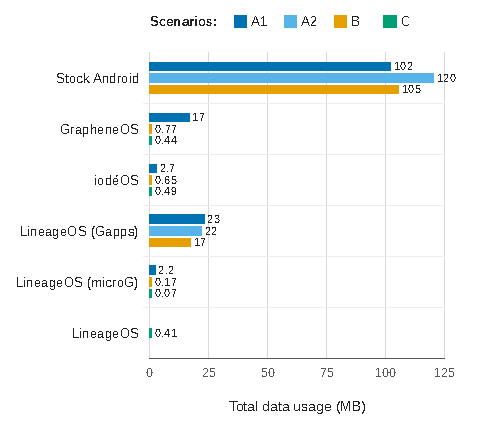
\includegraphics[width=\columnwidth]{images/all-tasks-data-usage-acm.pdf}
	\caption{Total data usage aggregated across all measurement tasks. Scenario applicability varies by system.} \label{fig-all-tasks-chart}
\end{figure}

\begin{figure}
	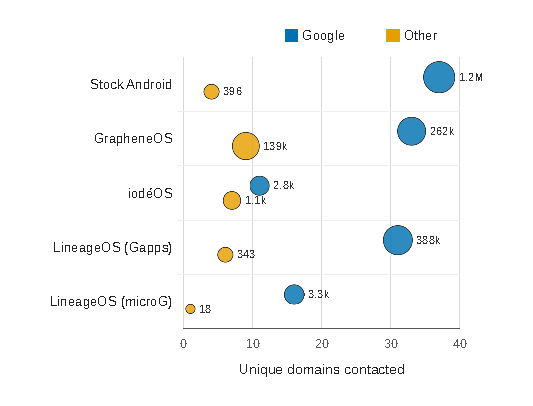
\includegraphics[width=\columnwidth]{images/os-domains-packets-acm.eps}
	\caption{Domains contacted in Scenario A1 aggregated for all tasks, grouped by operating system and by Google-related and other endpoints. Bubble size represents the total number of packets exchanged with each group. Vanilla LineageOS was omitted due to lack of available scenarios} \label{fig-domains-chart}
\end{figure}

Figure~\ref{fig-domains-chart} presents the domain-level distribution of network traffic. Stock Android contacts the most Google-related domains. iod\'eOS and LineageOS contact fewer servers overall. iod\'eOS also relies on some Mozilla infrastructure not present in other systems.

Table~\ref{tab:domains-mechanisms} shows the infrastructure dependencies for core system functions. LineageOS remains closest to stock Android, relying entirely on Google servers. iod\'eOS adopts an intermediate position, while GrapheneOS demonstrates the strongest de-Googling, substituting all three functions with its own or independently operated infrastructure.

Beyond aggregate traffic measurements, we were able to decrypt and analyze some payloads. A subset of these observations comes from earlier experiments performed on Android 14, because the Frida-based method was unsuccessful on Android 16.

Android's check-in mechanism transmits actual IMEI, MAC address, and hardware serial number to Google, while microG generates randomized, rotating identifiers (IMEI consistently prefixed with \texttt{35503104}, MAC addresses with OUI \texttt{b4:07:f9}). The Android ID field in microG requests is frequently empty or zeroed. The Google Advertising ID (ADID), formatted as a UUID, was observed in multiple requests on stock Android. This value remained constant across different requests, confirming its persistence as a cross-application tracking mechanism. After a manual reset in system settings, the ADID was transmitted as all zeros, indicating the identifier was actually cleared. We observed requests to \textit{app-measurement.com} on systems with Google services present, containing application package names, installation sources, versions, and the system theme preference.

When enabled, microG performs network geolocation without Google infrastructure by querying a selected provider, in our case \textit{api.position.xyz}. The request transmits nearby cell towers and returns approximate coordinates. We compared Google Play Store with Aurora Store (a popular application source in alternative Android distributions) by downloading the same application from each platform. Both stores retrieved identical packages from the same Google CDN infrastructure. However, the Play Store generated 106 requests, while Aurora Store produced 93.

In addition to network-level observations, Google Takeout\footnote{\url{https://takeout.google.com/}} was used to download data associated with test accounts for different Google services implementations. For every logged-in system, a corresponding entry appeared in \texttt{devices.json}, including device model, OS version, country, language, registration timestamp, and last activity time. However, the depth of telemetry varied considerably across configurations, as summarized in Table~\ref{tab:takeout-comparison}.

\begin{table}
	\caption{Domains observed for connectivity check, remote provisioning, and location assistance.}
	\label{tab:domains-mechanisms}
	
	\footnotesize
	\begin{tabular}{@{}p{0.11\columnwidth}p{0.3\columnwidth}p{0.25\columnwidth}p{0.22\columnwidth}@{}}
		\toprule
		System & Connectivity check& Provisioning & Location \\
		\midrule
		Stock & \url{connectivitycheck.gstatic.com} & -- & \url{supl.google.com}, \url{agnss.goog} \\
		Lineage & \url{connectivitycheck.gstatic.com} & \url{remoteprovisioning.googleapis.com} & \url{supl.google.com}, \url{agnss.goog} \\
		iod\'eOS & \url{captiveportal.kuketz.de} & \url{remoteprovisioning.googleapis.com} & \url{supl.google.com} \\
		Graphene & \url{connectivitycheck.grapheneos.network} & \url{remoteprovisioning.grapheneos.org} & \url{gs-loc.apple.grapheneos.org} \\
		\bottomrule
	\end{tabular}
\end{table}

\begin{table}
	\caption{Comparison of Google Takeout data across Android configurations.}
	\label{tab:takeout-comparison}

	\footnotesize
	\begin{tabular}{@{}p{0.25\columnwidth}p{0.23\columnwidth}p{0.20\columnwidth}p{0.20\columnwidth}@{}}
		\toprule
		System & Device IDs & Apps & Pixel telem. \\
		\midrule
		Stock Android & IMEI, serial & Extensive & Full \\
		Lineage (Gapps) & IMEI, serial & Extensive & Reduced \\
		Lineage (microG) & -- & -- & -- \\
		GrapheneOS & Falsified serial & 4 apps & -- \\
		\bottomrule
	\end{tabular}
\end{table}
\section{Conclusion}

Our evaluation demonstrates that alternative Android distributions significantly reduce unsolicited data transmissions, offering privacy protections that standard stock Android settings cannot replicate. Ultimately, the choice depends on the user's specific privacy and usability needs. It is a preliminary study and future research could extend the measurement period and conduct repeated trials to better isolate systematic behavior from transient network variations.

\bibliographystyle{ACM-Reference-Format}
\bibliography{refs}

\end{document}
